\label{cap:materiales}

\section{Conjuntos de datos}

En este trabajo se utilizaron dos conjuntos de datos de resonancia magnética de rodilla. El primero fue \textbf{MRNet}, empleado como dominio principal para el entrenamiento, validación y prueba interna de los modelos. El segundo fue un conjunto externo procedente del Hospital Clínico Universitario de Rijeka (Croacia) \cite{stajduhar2017semi}, utilizado para estudiar la generalización fuera del dominio original y realizar un experimento posterior de adaptación de dominio.

\subsection{MRNet}

MRNet es un dataset público desarrollado por la Escuela de Medicina de la Universidad de Stanford \cite{bien2018deep}. Contiene estudios de resonancia magnética de rodilla etiquetados para distintas patologías musculoesqueléticas, incluyendo roturas del ligamento cruzado anterior.

Cada estudio está compuesto por tres series tridimensionales correspondientes a los planos anatómicos estándar:

\begin{itemize}
    \item \textbf{Plano sagital}
    \item \textbf{Plano coronal}
    \item \textbf{Plano axial}
\end{itemize}

La Figura~\ref{fig:planos_ejemplo} muestra un ejemplo de los tres planos para un mismo estudio con rotura del LCA.

\begin{figure}[H]
\centering
\begin{minipage}{0.31\textwidth}\centering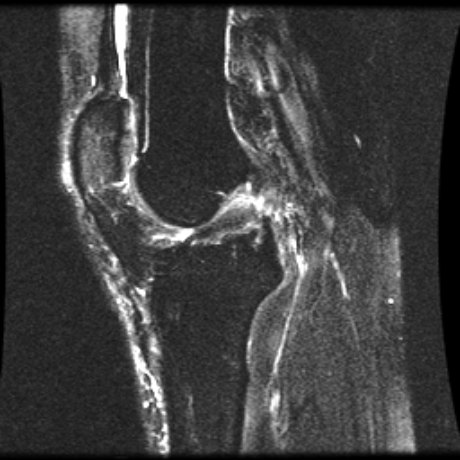
\includegraphics[width=\linewidth]{figs/plano_sagital.png}\\[2pt]\small Sagital\end{minipage}\hfill
\begin{minipage}{0.31\textwidth}\centering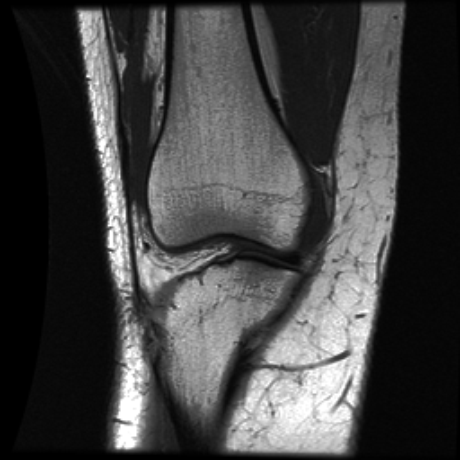
\includegraphics[width=\linewidth]{figs/plano_coronal.png}\\[2pt]\small Coronal\end{minipage}\hfill
\begin{minipage}{0.31\textwidth}\centering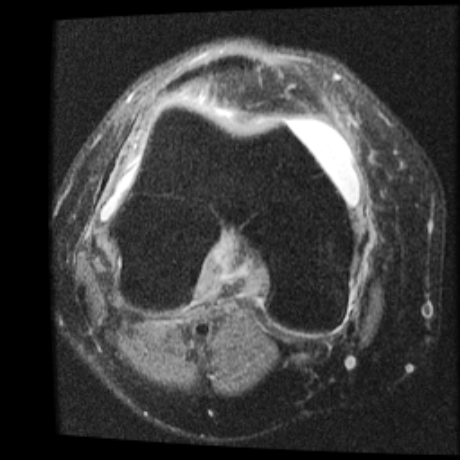
\includegraphics[width=\linewidth]{figs/plano_axial.png}\\[2pt]\small Axial\end{minipage}
\caption{Ejemplo de los tres planos anatómicos de un mismo estudio de RM de rodilla con rotura del LCA (MRNet).}
\label{fig:planos_ejemplo}
\end{figure}

Con el objetivo de evitar fuga de información (\textit{data leakage}), las particiones de entrenamiento, validación y prueba se realizaron a nivel de paciente.

\begin{table}[H]
\centering
\small
\caption{Distribución de casos clínicos empleados en el estudio.}
\label{tab:datos}
\begin{tabularx}{\textwidth}{
>{\raggedright\arraybackslash}X
>{\centering\arraybackslash}m{1.8cm}
>{\centering\arraybackslash}m{1.8cm}
>{\centering\arraybackslash}m{1.8cm}
>{\centering\arraybackslash}m{2cm}
}
\toprule
\textbf{Conjunto} &
\textbf{Casos} &
\textbf{LCA (+)} &
\textbf{Control (-)} &
\textbf{Prevalencia} \\
\midrule

Entrenamiento &
875 &
183 &
692 &
20.91\% \\

Validación &
188 &
36 &
152 &
19.15\% \\

Prueba &
187 &
43 &
144 &
22.99\% \\

\midrule
\textbf{Total} &
\textbf{1250} &
\textbf{262} &
\textbf{988} &
\textbf{20.96\%} \\

\bottomrule
\end{tabularx}
\end{table}

La distribución de clases presenta un desbalance considerable, reflejando una situación representativa del entorno clínico real, donde las lesiones completas del LCA representan una proporción minoritaria respecto al total de estudios de RM de rodilla.

\subsection{Conjunto externo de Croacia}

Además de MRNet, se utilizó un conjunto externo de resonancias magnéticas de rodilla procedente del Hospital Clínico Universitario de Rijeka (Croacia), publicado por {\v{S}}tajduhar et al.\ \cite{stajduhar2017semi}. Este conjunto permitió evaluar la robustez de los modelos ante un cambio de dominio, es decir, ante posibles diferencias en población, protocolo de adquisición, escáner o distribución de las imágenes respecto al conjunto original.

El conjunto de Croacia contiene 917 estudios. A diferencia de MRNet, su anotación original distingue tres grados de afectación del LCA: ligamento intacto (690 estudios), parcialmente roto (172 estudios) y completamente roto (55 estudios). Dado que en este trabajo la tarea se formula como una clasificación binaria (presencia o ausencia de rotura), las categorías de rotura parcial y rotura completa se unificaron en una única clase positiva, resultando en 690 casos sin rotura y 227 casos con rotura. Esta decisión sigue el criterio empleado por los propios autores del conjunto \cite{stajduhar2017semi} y permite una comparación directa con el etiquetado binario de MRNet, si bien debe tenerse en cuenta que la inclusión de roturas parciales introduce casos de mayor sutileza diagnóstica en la clase positiva. En primer lugar, se empleó para una validación externa \textit{zero-shot}, evaluando los modelos entrenados sobre MRNet sin reajustar sus pesos. Posteriormente, se utilizó para un experimento de \textit{fine-tuning} con el objetivo de analizar si la adaptación al nuevo dominio podía mejorar el rendimiento o modificar la calibración del clasificador.

Para el experimento de adaptación de dominio, el conjunto de Croacia se dividió en 641 casos de entrenamiento, 138 de validación y 138 de prueba. En el subconjunto de prueba había 104 casos sin rotura y 34 casos con rotura del LCA. Igual que en MRNet, las particiones se realizaron a nivel de paciente para evitar fuga de información entre conjuntos.

\section{Representación y preprocesamiento de datos}

Cada estudio de RM puede representarse matemáticamente como un volumen tridimensional:

\begin{equation}
V \in \mathbb{R}^{S \times H \times W}
\end{equation}

\noindent donde $S$ representa el número de cortes del volumen, mientras que $H$ y $W$ corresponden a la resolución espacial de cada corte.

Las intensidades de píxel fueron normalizadas mediante escalado Min-Max:

\begin{equation}
x_{\text{norm}} =
\frac{x - x_{\text{min}}}
{x_{\text{max}} - x_{\text{min}}}
\end{equation}

Posteriormente, todas las imágenes fueron redimensionadas a una resolución espacial de $224 \times 224$ píxeles. Dado que los modelos empleados utilizan pesos preentrenados en ImageNet, las imágenes monocanal fueron replicadas sobre tres canales de entrada.